\chapter{Background}

\section{Multi-Agent Oriented Programming}
The concept of a software agent can be traced back to the early days of research into Distributed AI in the 1970s when Carl Hewitt proposed the concurrent Actor model.
In his paper, he introduced the concept of a self-contained, interactive, and concurrently-executing object which he termed ``actor''.
The latter is a computational agent with a mail address and behavior. Actors can communicate by message-passing and carry out their actions concurrently. \cite{hewitt1977viewing}

\subsection{What is an Agent?}
The term ``agent'' quickly spread to heterogeneous research fields; therefore, there is no commonly agreed definition for it.
However, a generally accepted description of what an agent is is the following by Wooldridge \cite{490039}:
\begin{quote}
    \textit{An agent is a self-contained program capable of controlling its own decision-making and acting, based on its perception of its environment, in pursuit of one or more objectives.}
\end{quote}
To sum up, we can identify a set of features that an agent should possess:
\begin{itemize}
    \item \textbf{Autonomy}: agents should be able to perform most of their tasks without the direct intervention of humans or other agents, and they should encapsulate control over their actions and internal state
    \item \textbf{Social ability}: agents should be able to interact with each other and possibly humans to complete their tasks.
    \item \textbf{Responsiveness} (situatedness): agents should perceive their environment and respond to changes in it.
    \item \textbf{Proactiveness}: agents should exhibit opportunistic, goal-directed behavior and take the initiative when appropriate.
\end{itemize}

During the first years, the research concentrated on interaction and communication among agents, decomposition and distribution of tasks, and coordination and cooperation.
The goal was to specify, analyze, design, and integrate systems containing multiple collaborative agents.

\subsection{Multi-Agent Systems}
Multi-Agent Systems have been studied as a per se field since the 1980s and gained widespread recognition in the 1990s.
Since then, international interest in the topic has grown enormously as agents are considered an appropriate paradigm to exploit the possibilities presented by massive open distributed systems.
Moreover, MAS seem to be a natural metaphor for understanding and building a wide range of what we might call \textit{artificial social systems}. \cite{wooldridge2009introduction}

According to the \textit{Alan Turing Institute} \cite{turing}
\begin{quote}
    \textit{A Multi-Agent System consists of multiple decision-making agents which interact in a shared environment to achieve common or conflicting goals.}
\end{quote}

\begin{figure}[H]
    \centering
    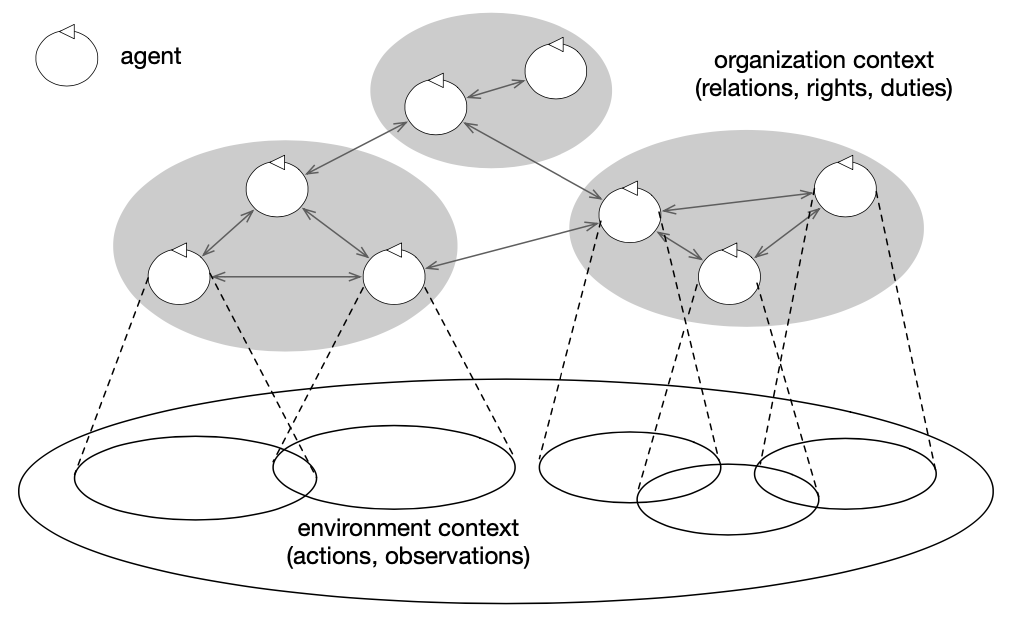
\includegraphics[width=0.9\linewidth]{images/multi-agent-systems.png}
    \caption{A representation of Multi-Agent Systems. \cite{jennings2000agent}}
    \label{fig:multi-agent-systems}
\end{figure}
As it can be noticed in \cref{fig:multi-agent-systems}, MAS are composed of the environment and agents existing within it that are bonded by relations.

\subsubsection{Environment}
The environment in MAS presents two facets:
\begin{itemize}
    \item \textit{The environment as the ``external world''}.
    Agents become aware of the context they are immersed in and its dynamics by perceiving the environment through sensors.
    Moreover, they pursue their goals through actions performed by actuators that aim at modifying the environment, eventually reaching the latter's desired state.
    \item \textit{The environment as a medium for coordination}
\end{itemize}

\section{Hypermedia Multi-Agent Systems}
\section{Organizations in Multi-Agent Systems}
